\documentclass[12pt,aspectratio=169]{beamer}

\usetheme{metropolis}
\setbeamertemplate{bibliography item}{\insertbiblabel}
\usepackage{xcolor}
\usepackage{appendixnumberbeamer}
\usepackage{verbatim}
\usepackage{caption}
\usepackage{minted}
\setsansfont[BoldFont={Fira Sans Bold}, ItalicFont={Fira Sans Italic}]{Fira Sans Regular}
\usepackage[backend=biber,style=ieee]{biblatex}
\bibliography{references}
\graphicspath{{./figs/}}
\setlength{\belowcaptionskip}{-10pt}
\definecolor{darkred}{RGB}{178,34,34}
%\setbeamercolor{normal text}{fg=black}
%\usebeamercolor[fg]{normal text}
\setbeamersize{text margin left=5mm,text margin right=7mm}

\title{DRILLS: Debugging RTL Intelligently with Localization from Long Simulation}
\subtitle{{\small Specification mining using waveform dumps from long-running FPGA emulation to localize bugs in complex digital designs.}}
\author{Donggyu Kim \& Vighnesh Iyer}
\date{Final Presentation: 5/6/2019}

\begin{document}
\begin{frame}
    \maketitle
\end{frame}

\begin{frame}{Problem Definition}
  \begin{itemize}
  \setlength\itemsep{0.75em}
    \item Higher RTL design productivity (Chisel, HLS) enables more complex digital designs (e.g. BOOM-v2), but complex designs usually contain subtle bugs
    \item Tricky bugs only manifest after trillions of cycles (e.g. running SPEC2017), as high-level assertion failures, hanging, or termination with errors
    \begin{itemize}
      \setlength\itemsep{0.5em}
      \item {\small e.g. pipeline hung, invalid writeback in ROB (see DESSERT [FPL’18])}
    \end{itemize}
    \item Even with a waveform, it is very laborious or even impossible to figure out where and when the bug originated.
    \item \textbf{Problem}: given many error-free traces and one error containing trace, localize the likely bug location by module or line of RTL and find the fine-grained implicit properties which were violated.
  \end{itemize}
\end{frame}

\begin{frame}{Hypothesis}
  \begin{itemize}
    \setlength\itemsep{0.75em}
    \item \textit{We believe} if a test fails after billions of cycles on a mature RTL design, an assumption the designer made was violated somewhere and at some time
      \begin{itemize}
        \item The final test failure could have sprung from latent state that was corrupted billions of cycles ago
      \end{itemize}
    \item The designer’s \textit{assumptions} can be extracted from waveforms with ‘normal’ activity using specification mining
    \item We can add these mined specifications (as assertions) to the design and replay the failing test to catch a faulty assumption \textbf{earlier and with greater locality}
  \end{itemize}
\end{frame}

\begin{frame}{Goals/Approach}
  \begin{itemize}
    \setlength\itemsep{0.75em}
    \item We want a specification mining system that can address:
      \begin{itemize}
        \item Automated suite of regression assertions
        \item Early bug detection and localization on long-running tests
        \item Starting point for formal specs of a design
      \end{itemize}
    \item We aim to first replicate Li's spec mining engine and templates, and apply it to \texttt{riscv-mini} on short ISA tests to detect user-inserted bugs
    \item Next, we will apply the spec mining engine to \texttt{rocket-chip} and try it on longer traces
  \end{itemize}
\end{frame}

\begin{frame}{Proposed Approach}
  \begin{figure}
    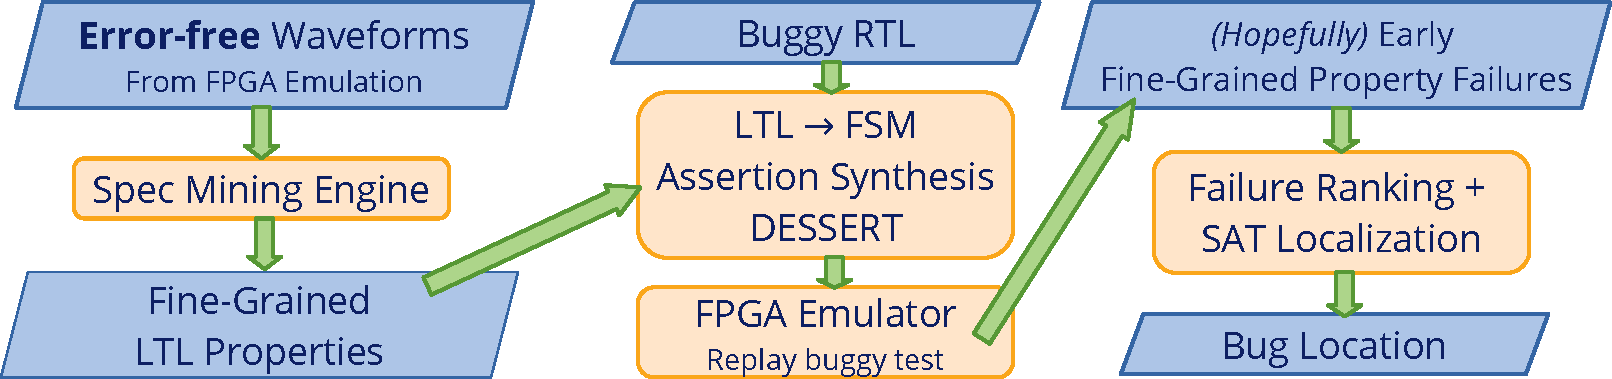
\includegraphics[width=\textwidth]{proposed_approach.pdf}
  \end{figure}
\end{frame}

\begin{frame}{LTL (Linear Temporal Logic)}
  \begin{itemize}
    \item {\small LTL is a logic for defining \textit{properties} over \textit{traces} of \textit{atomic propositions}}
    \item {\small In the digital design context:}
    \begin{itemize}
      \item {\footnotesize A trace is a signal (registers/wires) sampled at rising clock edges; traces are of finite length (not true for LTL in general)}
      \item {\footnotesize Atomic propositions (AP) are functions over signal(s) that evaluate to boolean values}
    \end{itemize}
  \end{itemize}
  {\footnotesize
  Trace of signal $a = \tau_a = \{0, 1, 1, 1, 0\}$

  Trace of signal $b = \tau_b = \{0, 100, 200, 300, 0\}$

  AP $x = f(a) = (a == 1)$, AP $y = f(b) = (b >= 200)$

  Trace of AP $x = \tau_x = \{0, 1, 1, 1, 0\}$

  Trace of AP $y = \tau_y = \{0, 0, 1, 1, 0\}$
  }
\end{frame}

\begin{frame}{LTL Logical Operators}
  \begin{itemize}
    \setlength\itemsep{0.75em}
    \item An LTL formula $\phi$ is defined over a trace of tuples of APs.
      \begin{itemize}
        \item {\small Consider the last example: $\tau = \{( ), (x), (x, y), (x, y), ( )\}$}
      \end{itemize}
    \item An AP on its own is a valid LTL formula
      \begin{itemize}
        \item {\small For example $\phi = x$. This formula is satisfied if the first element of the trace contains the AP.}
      \end{itemize}
    \item APs can be composed with simple logic operators ($\lnot, \land, \lor, \rightarrow$) to form another valid LTL formula
      \begin{itemize}
        \item {\small For example $\phi = (\lnot x \lor y)$. This formula is satisfied if the first element of the trace contains the AP.}
      \end{itemize}
  \end{itemize}
\end{frame}

\begin{frame}{LTL Temporal Operators}
  \begin{itemize}
    \item There are 4 (commonly used) LTL temporal operators (let $p, q$ be APs or LTL formulas):
      \begin{itemize}
        \setlength\itemsep{0.5em}
        \item $\mathbf{G} p$ (\textit{globally}, $p$ must hold for the entire trace) \\
          {\small $\quad \{(p), (p), (p,q), (p), (p)\}$}
        \item $\mathbf{F} p$ (\textit{eventually}, $p$ must eventually hold at some point)\\
          {\small $\quad \{(), (), (q), (q,p), (p)\}$}
        \item $\mathbf{X} p$ (\textit{next}, $p$ must hold in the next timestep) \\
          {\small $\quad \{(), (p), (p), (q), ()\}$}
        \item $p \mathbf{U} q$ (\textit{until}, $p$ must hold until $q$ holds) \\
          {\small $\quad \{(p), (p), (p, q), (q), ()\}$}
      \end{itemize}
    \item Common combinations include $\mathbf{G} \mathbf{F} p$ ($p$ holds infinitely often) and $\mathbf{FG} p$ (once $p$ holds, it holds forever)
  \end{itemize}
\end{frame}

\begin{frame}{Hardware Idioms in LTL}
Many common temporal RTL patterns are expressible in LTL.
  \begin{itemize}
    \setlength\itemsep{0.75em}
    \item There should eventually be a response after a request is dispatched \\
      $\quad \mathbf{G}\, (\text{req} \rightarrow \mathbf{XF}\, \text{resp})$
    \item The memory bus should respond in 2 cycles \\
      $\quad \mathbf{G}\, (\text{req} \rightarrow \mathbf{XX}\, \text{resp})$
    \item \texttt{IrrevocableIO} should keep valid high until ready has been asserted \\
      $\quad \mathbf{G}\, (\text{valid} \rightarrow \mathbf{X}\, (\text{valid}\, \mathbf{U}\, \text{ready}))$
    %\item \texttt{IrrevocableIO} should not touch \texttt{bits} after valid goes high until the transaction is accepted \\
      %$\quad \mathbf{G}\, (\text{valid} \rightarrow \
    \item After a transaction, the slave should be ready again within 2 cycles \\
      $\quad \mathbf{G}\, ((\text{valid} \land \text{ready}) \rightarrow (\mathbf{X}\, \text{ready} \lor \mathbf{XX}\, \text{ready}))$
  \end{itemize}
\end{frame}

\begin{frame}{LTL Templates}
There are several LTL formulas that can be 'templated' to be filled in with concrete signals from a design.
  \begin{itemize}
    \item Alternating: $a\, \mathbf{A}\, b$ \\
      $\quad$ Example: $\{(a), (a), (b), (a), (b)\}$
    \item Until: $\mathbf{G}\, (a \rightarrow \mathbf{X}\, (a\, \mathbf{U}\, b))$
    \item Next: $\mathbf{G}\, (a \rightarrow \mathbf{X}\, b)$
    \item Eventual: $\mathbf{G}\, (a \rightarrow \mathbf{X F}\, b)$
  \end{itemize}
These property templates are from Wenchao Li's thesis. We implement these templates in the spec mining engine.
\end{frame}

\begin{frame}{Delta Traces}
  \begin{itemize}
    \setlength\itemsep{0.75em}
    \item Signals in RTL designs aren't APs on their own, so we use delta traces to capture \textit{changes} in a signal from one timestep to the next
    \begin{itemize}
      \item Trace of signal $a = \tau_a = \{0, 1, 1, 1, 0\}$
      \item Trace of signal $b = \tau_b = \{0, 100, 200, 300, 0\}$
      \item Delta trace of signal $a = \tau_{\Delta a} = \{0, 1, 0, 0, 1\}$
      \item Delta trace of signal $b = \tau_{\Delta b} = \{0, 1, 1, 1, 1\}$
    \end{itemize}
    \item VCD (value change dump) files already store delta traces in compressed format
    \item Custom user-defined events can be used to construct AP traces (such as AP $f(r,v) = r \land v$ for ready/valid interfaces)
  \end{itemize}
\end{frame}

\begin{frame}{Specification Mining}
  \begin{itemize}
    \setlength\itemsep{0.75em}
    %\item Using the user-defined LTL templates, substitute in all possible combinations of delta traces and check whether they hold
    \item We use a tool (SPOT) to construct a Buchi-automaton that acts like an LTL property monitor
    \begin{figure}
      \centering
      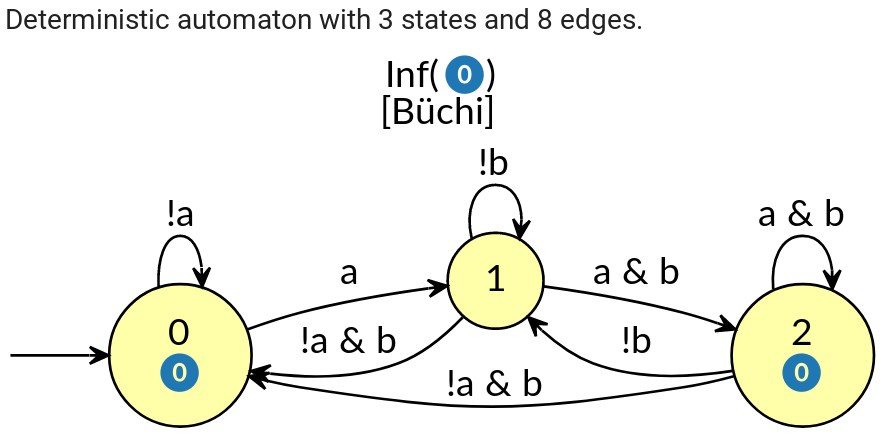
\includegraphics[width=0.3\textwidth]{spot.png}
      \caption{Monitor for $\mathbf{G}\, (a \rightarrow \mathbf{XF}\, b)$}
    \end{figure}
  \item We use a naive algorithm ($\mathcal{O}(n!)$) to plug in delta traces to the template and check whether the property holds.
      \begin{itemize}
        \setlength\itemsep{0.5em}
        \item We use the sparsity of delta traces to perform spec mining efficiently
        \item We restrict the signal permutations under consideration to be within 1 module
      \end{itemize}
  \end{itemize}
\end{frame}

\begin{frame}[fragile]{As of 2 Weeks Ago}
  \begin{itemize}
    \item {We have a spec miner in Python that can evaluate the 'alternating' and 'next' templates using VCD files as input}
    \item {It works on \texttt{chisel-examples} and \texttt{riscv-mini} (and \texttt{rocket-chip} if only 1 clock is considered)}
  \end{itemize}
  {Here's an example property mined from \texttt{riscv-mini}}
  \begin{minted}[breaklines, fontsize=\footnotesize]{text}
    Next: [['TOP.Tile.core.dpath.csr_io_stall', 'TOP.Tile.core.dpath.stall', 'TOP.Tile.core.dpath.csr.io_stall'], ['TOP.Tile.icache.is_idle']]
  \end{minted}

  \begin{figure}
    \centering
    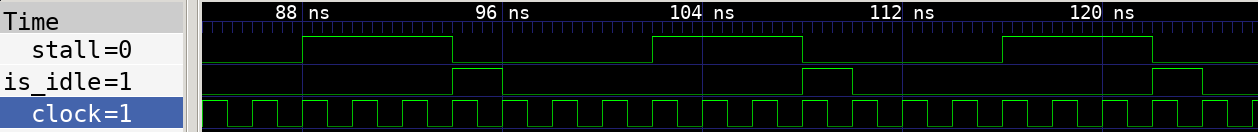
\includegraphics[width=0.7\textwidth]{waveform.png}
  \end{figure}
\end{frame}

\begin{frame}[fragile]{As of 2 Weeks Ago: Bugs Everywhere!}
  \begin{minted}[breaklines, fontsize=\footnotesize]{text}
    Next: [['TOP.Tile.core.dpath.csr_io_stall', 'TOP.Tile.core.dpath.stall', 'TOP.Tile.core.dpath.csr.io_stall'], ['TOP.Tile.icache.is_idle']]
  \end{minted}

  \begin{figure}
    \centering
    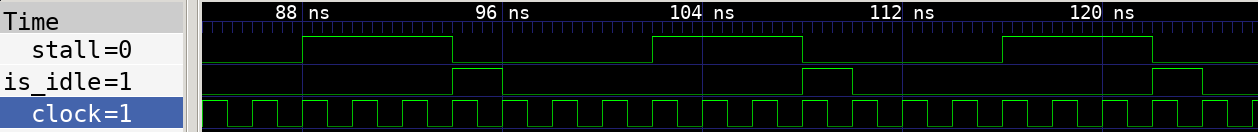
\includegraphics[width=0.7\textwidth]{waveform.png}
  \end{figure}

  Look closely, the waveform doesn't match the property template!
\end{frame}

\begin{frame}{Current Status}
  \begin{itemize}
    \item Support for all 4 property templates and some tests
    \item Support for module-level mining and deduplication
    \item Merging mined properties from several VCDs
    \item Checking property sets against VCDs
    \item Notions of falsifiability, falsification, and support
    \item Automated mine and check flow for \texttt{riscv-mini}
  \end{itemize}
\end{frame}

\begin{frame}[fragile]{Mining on a store ISA test}
  \begin{minted}[breaklines, fontsize=\scriptsize]{text}
python miner.py --start-time 12 --signal-bit-limit 4 rv32ui-p-sw.vcd
Top 10 properties:
Until TOP.Tile.core.ctrl.io_A_sel -> TOP.Tile.core.ctrl_io_imm_sel, support: 331
Next TOP.Tile.core.dpath.brCond.eq -> TOP.Tile.core.dpath.brCond.neq, support: 291
Next TOP.Tile.core.dpath.brCond.neq -> TOP.Tile.core.dpath.brCond.eq, support: 291
Eventual TOP.Tile.core.ctrl_io_imm_sel -> TOP.Tile.core.dpath.regFile.io_wen, support: 248
Next TOP.Tile.core_io_icache_req_valid -> TOP.Tile.icache.is_idle, support: 233
Next TOP.Tile.core_io_icache_req_valid -> TOP.Tile.icache.is_read, support: 233
Until TOP.Tile.core_io_icache_req_valid -> TOP.Tile.icache.state, support: 233
Until TOP.Tile.icache.is_idle -> TOP.Tile.icache.is_read, support: 233
  \end{minted}
\end{frame}

\begin{frame}[fragile]{Mining on a jump ISA test}
  \begin{minted}[breaklines, fontsize=\scriptsize]{text}
python miner.py --start-time 12 --signal-bit-limit 4 rv32ui-p-jal.vcd
Until TOP.Tile.core.dpath.io_ctrl_A_sel -> TOP.Tile.core.dpath_io_ctrl_imm_sel, support: 37
Until TOP.Tile.core.ctrl.io_wb_sel -> TOP.Tile.core.dpath_io_ctrl_imm_sel, support: 34
Next TOP.Tile.core.dpath_io_ctrl_inst_kill -> TOP.Tile.core.ctrl_io_pc_sel, support: 33
Next TOP.Tile.core.dpath_io_ctrl_inst_kill -> TOP.Tile.core.ctrl.io_wb_sel, support: 33
Next TOP.Tile.core.ctrl_io_pc_sel -> TOP.Tile.core.dpath_io_ctrl_inst_kill, support: 33
Next TOP.Tile.core.ctrl_io_pc_sel -> TOP.Tile.core.ctrl.io_wb_sel, support: 33
Next TOP.Tile.core.dpath.brCond.eq -> TOP.Tile.core.dpath.brCond.neq, support: 33
Next TOP.Tile.core.dpath.brCond.neq -> TOP.Tile.core.dpath.brCond.eq, support: 33
  \end{minted}
\end{frame}

\begin{frame}[fragile]{Bug Localization}
Can typos or copy/paste mistakes be caught?
  \begin{minted}{scala}
   io.csr_cmd := ctrlSignals(11)
-  io.illegal := ctrlSignals(12)
+  io.illegal := ctrlSignals(11)
  \end{minted}

  This caused a test to hang, so let's check if any mined specs were violated:
  \begin{minted}[breaklines, fontsize=\scriptsize]{text}
python checker.py --start-time 12 --signal-bit-limit 4 rv32ui-p-sub.vcd riscv_mini.props
ERROR on property Until TOP.Tile.core.dpath.csr.io_illegal -> TOP.Tile.icache.io_cpu_req_valid
ERROR on property Until TOP.Tile.core.dpath.csr.io_illegal -> TOP.Tile.icache.io_cpu_resp_valid
ERROR on property Until TOP.Tile.core.dpath.csr.io_illegal -> TOP.Tile.core.ctrl.io_A_sel
  \end{minted}
\end{frame}

\begin{frame}{Challenges}
  \begin{itemize}
    \setlength\itemsep{0.75em}
    \item Many of the specs are meaningless or require very specific behaviors to falsify
    \item Some of the specs can be statically inferred (like shift registers)
    \item These spec templates aren't sufficient to catch some typo bugs
    \item The VCD parser is too slow to run on longer traces like the RISC-V benchmarks
  \end{itemize}
\end{frame}

\begin{frame}{Current Status and Future Work}
  \begin{itemize}
    \setlength\itemsep{0.75em}
    \item We built a spec mining engine to replicate the prior work
    \item We applied the engine to \texttt{riscv-mini} and demonstrated its strengths and weaknesses
    \item There's a lot of future work in refining the spec templates and in software engineering
    \item The ultimate goal of applying this work to debug BOOM is a while away
  \end{itemize}
\end{frame}

%\renewcommand*{\bibfont}{\scriptsize}
%\printbibliography

\end{document}
